\paragraph{Compilazione questionario}

\subparagraph{Inizio questionario}

\label{Inizio questionario}

\begin{figure}[ht]
	\centering
	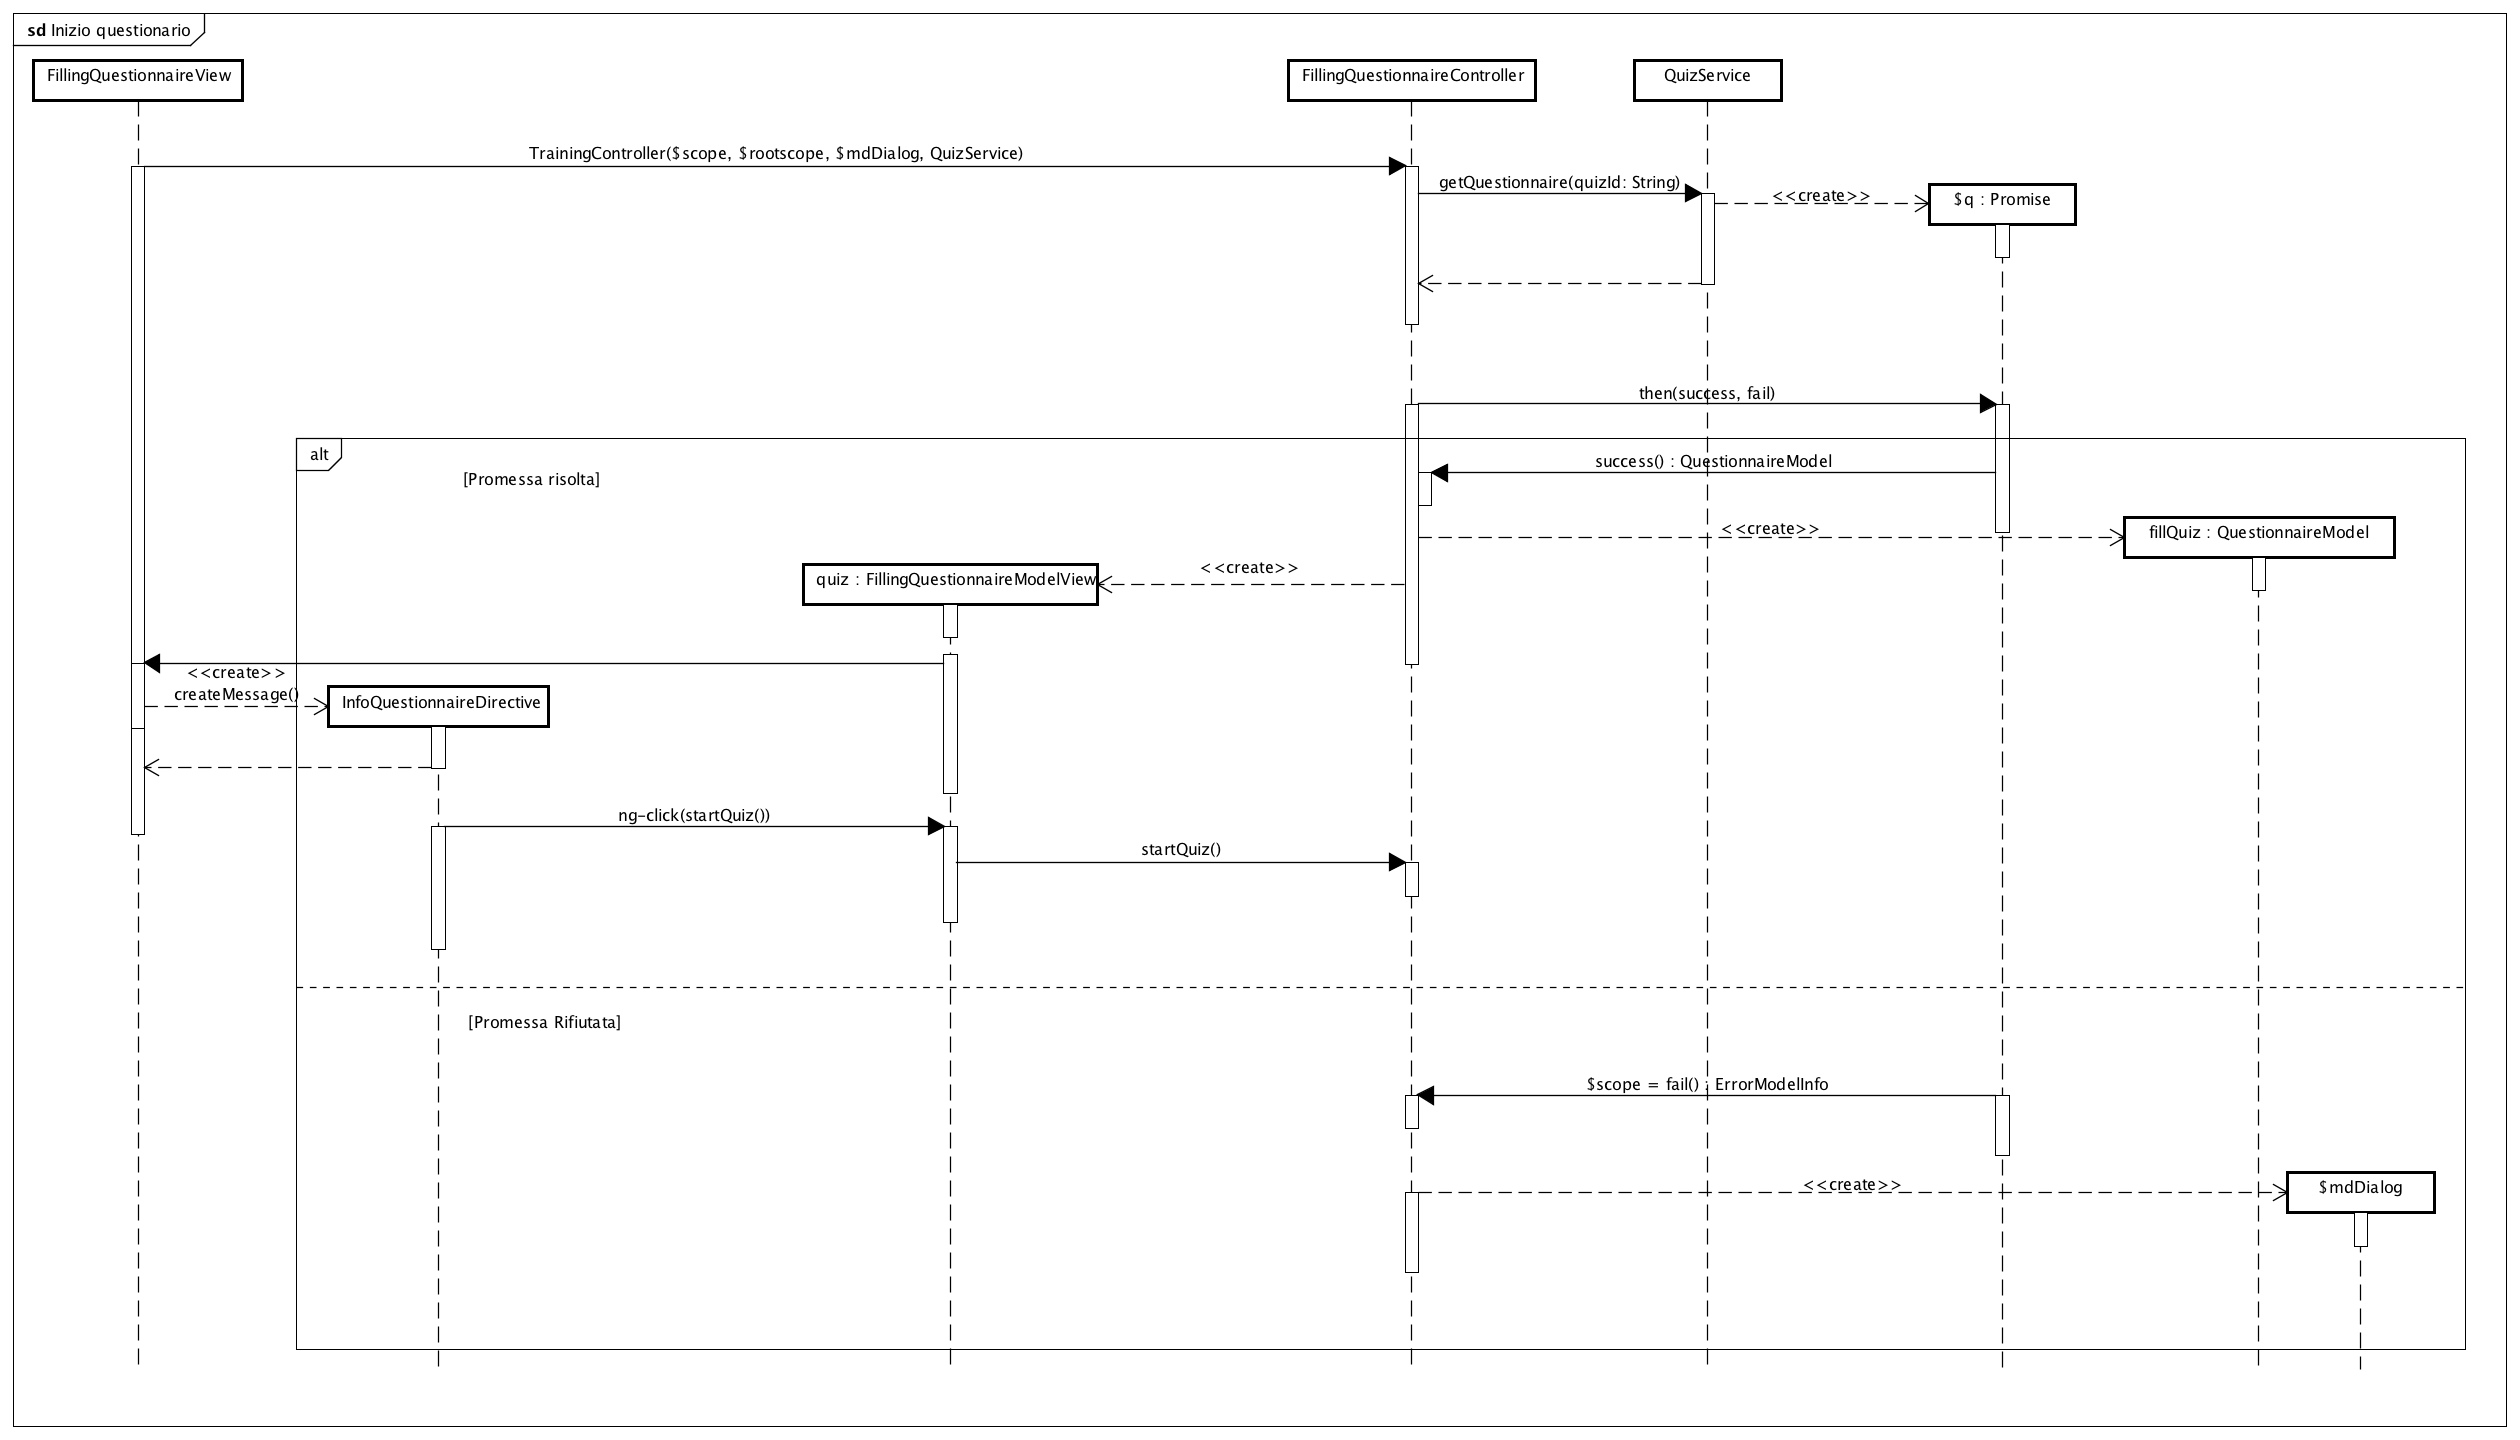
\includegraphics[scale=0.20,keepaspectratio]{UML/DiagrammiDiSequenza/Front-end/Quiz_start.png}
	\caption{Inizio questionario}
\end{figure} \FloatBarrier

Al caricamento della pagina di compilazione di un questionario, il\\ \texttt{FillingQuestionnaireController} attraverso il \texttt{QuestionnaireService} recupera dal back-end un oggetto di tipo \texttt{QuestionnaireModel}. Il \texttt{service\ped{G}} citato esegue questa operazione mediante l'utilizzo delle \texttt{promise\ped{G}}. Se questa verrà risolta popolerà l'oggetto presente nello \texttt{\$scope} di tipo \texttt{FillingQuestionnaireModelView}, così da mostrare nella \texttt{view\ped{G}} associata la pagina di inizio del questionario. Altrimenti verrà restituito un oggetto di tipo \texttt{ErrorInfoModel} che verrà visualizzato a video mediante un popup \texttt{\$mdDialog}. \\
L'utente mediante l'evento \texttt{ng-click} potrà dare inizio al questionario. 

\subparagraph{Composizione di una domanda}

Per comporre una domanda verrà eseguita la stessa sequenza di operazioni che sono presenti nella modalità allenamento. Eseguendo un loop sulla variabile di tipo \texttt{QuestionsModelView} precisamente sull'array \texttt{piecesOfQuestion}, per ogni pezzo di domanda verrà visualizzata la giusta direttiva così da comporre la domanda nella sua totalità.

\subparagraph{Risposta ad una domanda}

Per rispondere ad una domanda verrà eseguita la stessa sequenza di operazioni che sono presenti nella modalità allenamento.


